\chapter*{Introduction}
\addcontentsline{toc}{chapter}{Introduction}

Consider a simple\footnote{An undirected graph with no self loops and at most 1 edge between any two nodes} graph $G$. How many colours do you need to colour each edge such that no edges which touch
have the same colour? What if no edges which even touch some common edge can have the same colour?
Erd\H{o}s and Nešetřil conjectured that you only need $1.25\Delta(G)^2$ edges, but
the best known proof only shows an upper bound of $1.772\Delta(G)^2$ edges. In this thesis
we show how we can bring this bound down to $1.73\Delta(G)^2$ by introducing a new framework
which is a modification of the flag algebras framework.

\section*{Strong Edge Colouring}
\addcontentsline{toc}{section}{Strong Edge Colouring}

An edge colouring of a simple graph $G$ is an assignment $c\colon E(G) \to [k]$
for some $k\in\N$. Such a colouring is \textit{proper} if no two incident\footnote{Have a vertex in common}
edges are coloured the same.
A colouring is \textit{strong} if no edges which share a common incident edge are
coloured the same. Intuitively strong colouring requires edges at distance 1 to have distinct
colours and strong colouring extends this to distance 2.
In figure \ref{fig:proper-strong-example} we see an example of a non-proper colouring,
a proper (but not strong) colouring and a strong colouring of $C_5$.

\begin{figure}[h]
    \centering
    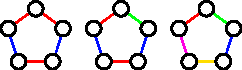
\includegraphics[scale=1.5]{proper-strong-example}
    \caption{Non-Proper, Proper \& Strong Edge Colourings}
    \label{fig:proper-strong-example}
\end{figure}

The \textit{chromatic index} of $G$, denoted $\chi'(G)$, is the minimum $k$ such that a proper edge
colouring of $G$ with $k$ colours exists. The \textit{strong chromatic index} $\chi'_s(G)$
is the corresponding minimum number of colours required for a strong edge colouring.

Vizing's theorem is a well known result which tells us $\chi'(G)$ almost exactly in terms of
the max degree of the graph $\Delta(G)$:
\begin{knowntheorem}[Vizing, 1965]
    $\Delta(G) \leq \chi'(G) \leq \Delta(G) + 1$.
\end{knowntheorem}
Erd\H{o}s and Nešetřil conjectured in 1985 \cite{faudreeInducedMatchingsBipartite1989} that
the strong chromatic index can also be bounded precisely by a function of the max degree:
\begin{conjecture}[Erd\H{o}s and Nešetřil]
    \label{conj:erdos-nesetril}
    $\chi'_s(G) \leq \frac{5}{4}\Delta(G)^2$.
\end{conjecture}
A greedy argument shows a bound of $\chi'(G) \leq 2\Delta(G)^2 + o(\Delta(G)^2)$ but it wasn't until
1997 that Molloy and Reed broke the $2\Delta(G)^2$ barrier \cite{molloyBoundStrongChromatic1997}.
A series of papers have since made progress on bringing this bound down closer to $\frac{5}{4}\Delta(G)^2$.

For $\Delta(G)$ large enough we have the following theorems:
\begin{enumerate}
  \item \textit{Molloy \& Reed, 1997} \cite{molloyBoundStrongChromatic1997}:
        $\chi'_s(G) \leq 1.998\Delta(G)^2$.
  \item \textit{Bruhn \& Joos, 2015} \cite{bruhnStrongerBoundStrong2018}:
        $\chi'_s(G) \leq 1.93\Delta(G)^2$.
  \item \textit{Bonamy, Perrett \& Postle, 2018} \cite{bonamyColouringGraphsSparse2018}:
        $\chi'_s(G) \leq 1.835\Delta(G)^2$.
  \item \textit{Hurley, de Verclos \& Kang, 2022} \cite{hurleyImprovedProcedureColouring2022}:
        $\chi'_s(G) \leq 1.772\Delta(G)^2$.
\end{enumerate}

In this thesis we will show how we brought this bound down even further to $1.73\Delta(G)^2$:
\begin{theorem}
    For $\Delta(G)$ large enough we have
    $\chi'_s(G) \leq 1.73\Delta(G)^2$.
\end{theorem}

The 1997 paper by Molloy \& Reed introduced a method for strong edge colouring we call the
\textit{2 step strategy}:
\begin{enumerate}
    \item Find an upper bound for the \textit{strong neighbourhood density} of $G$ in terms of
        $\Delta(G)$.
    \item Use a probabilistic colouring method which uses the previous bound to achieve a colouring
        with a low number of colours.
\end{enumerate}
This method has been modified by the papers which followed the Molloy \& Reed paper but this
strategy has remained the core idea. We will look at this strategy in more detail (including
defining strong neighbourhood density) in chapter TODO.
For this thesis we focus on the first step, using the second step as a black box.

% Given an edge $e\in E(G)$ we define the \textit{strong neighbourhood} of $e$,
% denoted $N_e(G)\subseteq E(G)$, to be all those edges $f\in E(G)$ which are at distance
% $\leq 2$ from $e$ (i.e. those relevant to strong edge colouring). Consider all pairs of
% distinct edges $f, f' \in N_e(G)$, some of these pairs of edges are themselves at distance $\leq 2$ to
% each other. Call the total number of such pairs $F(e)$ and note
% $F(e) \leq \binom{2\Delta(G)^2}{2}$.
% We define then the \textit{strong neighbourhood density}
% to be $F(e) / \binom{2\Delta(G)^2}{2}$ which is some real number $\in[0, 1]$.
% 
% If we think of the strong neighbourhood of $e$ as the set of edges which conflict with $e$
% in strong edge colouring, then the strong neighbourhood density at $e$ tells us how
% many of those edges which conflict with $e$ conflict with each other. Intuitively then
% the lower this number, the easier the colouring problem should be.

\section*{Flag Algebras}
\addcontentsline{toc}{section}{Flag Algebras}

Step 1 of the above method
asks us to find an upper bound on the strong neighbourhood density. Bounding densities
is a common problem in combinatorics and in 2007 Razborov \cite{razborovFlagAlgebras2007}
introduced a framework called \textit{flag algebras}
which can be used to prove asymptotic results about densities in various combinatorial structures.

These flag algebras are a syntactic tool which enables us to use computer search (in particular
the semidefinite method) in order to rigorously prove bounds on density functions.
They do this by capturing the algebraic relationships between the densities of small structures
into a symbolic algebra. Search methods can then apply standard algebraic identities and
tools such as Cauchy-Schwarz inequalities to prove bounds on density functions.

These flag algebras are defined very generally in terms of finite model theory in \cite{razborovFlagAlgebras2007} but we focus on their use with respect to simple graphs.

One might be tempted to try to apply these flag algebras directly to our strong neighbourhood
density problem but in practice this problem doesn't fit well into the flag algebra model.
Instead, this thesis introduces a modification of the flag algebra framework which can prove
results in problems of the flavour we are interested in.
